This section is focused on the audio properties of the PD patch and the control structures which operate them specifically. In addition to this, many different general-purpose control objects were created to streamline development. A full list is available in appendix \ref{x:glossary}, page \pageref{x:glossary}.
%
\begin{figure}[H]
	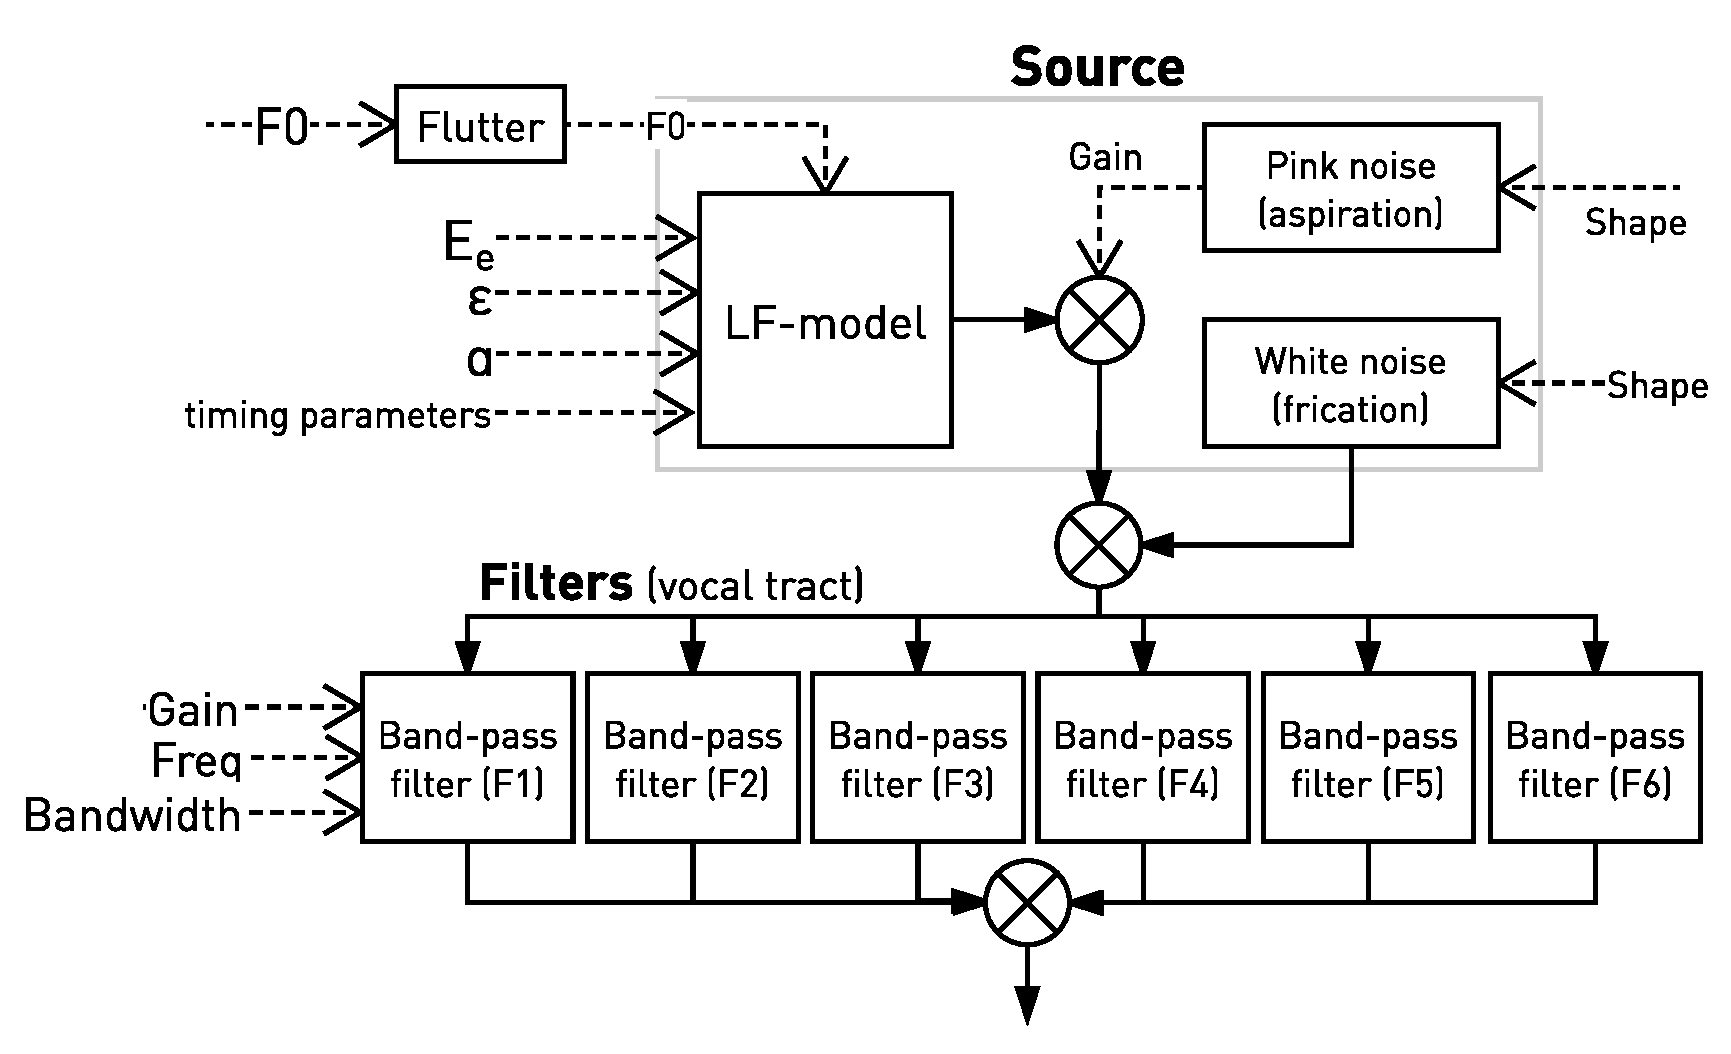
\includegraphics[width=0.5\textwidth]{signal_flow.pdf}
	\caption{Signal path diagram for the system. Audio signals are represented with black arrows, control signals are represented with dotted arrows.}
	\label{fig:signal_path}
\end{figure}
%
The synthesiser is configured as a parallel formant synthesiser with an adjustable LF-model of the glottal flow derivative as the sound source. Aspiration and frication noise are provided by two additional noise generators in the voice source. Pseudo-random flutter is implemented using Klatt's algorithm detailed in the previous section. The formants are modelled as band-pass filters with adjustable gain, centre frequency and bandwidth. The signal path is for this system is outlined in the signal flow diagram in Figure \ref{fig:signal_path} above.

In the top-level patch (\obj{synth}) the connecting edges of the objects are reserved only for audio signals to make the data flow clear (see Figure \ref{fig:top_level} below). Control signals are routed using message receivers.
%
\begin{figure}[H]
	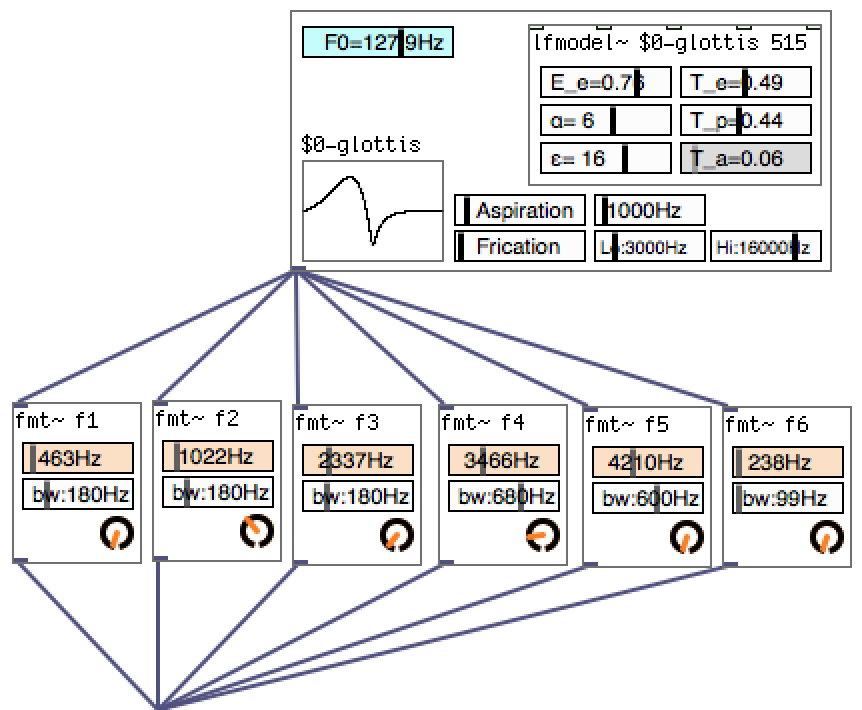
\includegraphics[width=0.5\textwidth]{top_level.png}
	\caption{Signal flow in \obj{synth}: from sound source through the vocal tract.}
	\label{fig:top_level}
\end{figure}
%
I initially used a large number of formants (10). This did create added realism but put a lot of burden when trying to make adjustments. Fant \cite{Fant1995} cites a formula
%
\begin{equation}
	m = F_s(l_e / c)
\end{equation}
%
which defines the minimum number of VTTF poles required to maintain correct spectral distribution for formant synthesis. Assuming an average male vocal tract length of $l_e=17.65\si{5cm}$ and a sampling rate of $F_s = \si{44100Hz}$ this indicates a need for 22 formants. This seems well beyond what is likely to be practical to implement in PD. To determine the resonant frequency of a particular formant Johnson \cite{Johnson2003} gives the formula
%
\begin{equation}
	F_n = \frac{(2n-1)c}{4l_e}
\end{equation}
%
which suggests that the tenth formant comes in at approximately 9.4kHz. As human hearing drops off after 10kHz I see no particular need to implement these higher formants in any case. For simplicity I reduced my system to five formants and added a sixth to model an additional prominent formant movement in the diphthong of my chosen word. I encourage the reader to experiment with selecting the bypass switch on the formants on my patch to hear what difference the formants above $F_3$ make.

In order to recreate the spectrum more precisely I had to use more configurable filters than the standard array of \obj{bp\~}, \obj{lop\~} and \obj{hip\~}. I found for the high and low-pass filters especially that the rolloff was too gradual to be of much use. Instead I used the built-in \obj{biquad\~} filter using \obj{bandpass} to calculate the coefficients for the formants. One problem with this is that if the control parameters are not interpolated smoothly enough it can create artefacts in the synthesis. However, reducing the time-grain for \obj{line} can introduce a lot of processor overhead. I tried to strike a balance. \obj{bandpass} specifies the bandwidth in octaves so I created some logic to convert to a bandwidth in Hertz to make adjustments more quickly. However, it does not map the centre frequency precisely because \obj{bandpass} sets the bandwidth logarithmically rather than linearly. 

A \obj{controller} patch—Figure \ref{fig:controller} below—has any array of buttons for different phonemes and words, and when they are pressed sends control messages to the vocal tract and voice source patches to configure them.
%
\begin{figure}[H] 
	\centering
	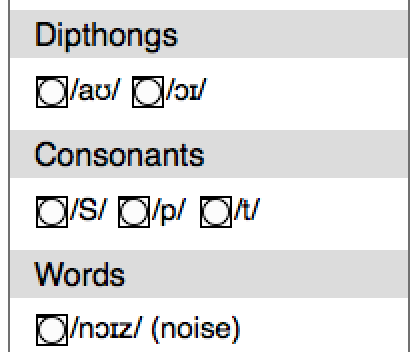
\includegraphics[height=3cm]{controller.png}
	\caption{A small section of the \obj{controller} patch showing how presets can be selected.}
	\label{fig:controller}
\end{figure}
%
Most control messages are terminated with a linear ramp time in ms. Sequencing chains of these events is handled with \obj{qlist} and a message delay pipe, see \obj{msgpipe} in appendix \ref{x:glossary} for more details.

I aimed to create a flexible synthesis system that could be configured rapidly. In the pursuit of naturalness it is equally important to have rapid turnaround of analysis of synthesis attempts, as there is a large element of trial and error without using more sophisticated techniques. To aid with this I created \obj{desk\`} to allow recording directly from the synthesiser as easily as possible (see Figure \ref{fig:desk} below). Once a location has been selected with the `eject' button, pressing record will record to that file until stop is pressed.
%
\begin{figure}[H]
	\centering
	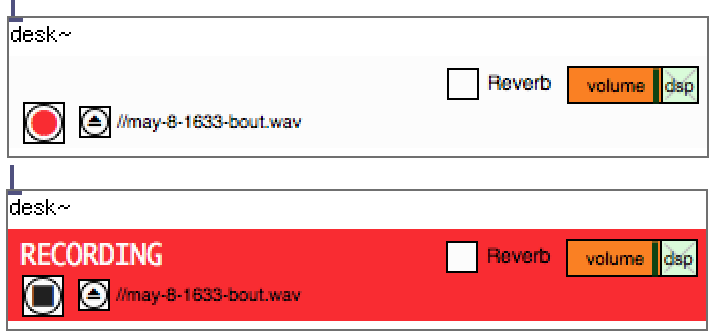
\includegraphics[width=0.39\textwidth]{desk.png}
	\caption{\obj{desk\~} object for rapidly saving samples for analysis when stopped (above) and recording (below).}
	\label{fig:desk}
\end{figure}
%